\documentclass[a4paper,11pt]{article}
\input{/home/tof/Documents/Cozy/latex-include/preambule_lua.tex}
\newcommand{\showprof}{show them}  % comment this line if you don't want to see todo environment
\fancyhead[L]{Produire un code correct}
\newdate{madate}{10}{09}{2020}
%\fancyhead[R]{\displaydate{madate}} %\today
%\fancyhead[R]{Seconde - SNT}
\fancyhead[R]{Première - NSI}
%\fancyhead[R]{Terminale - NSI}
\fancyfoot[L]{~\\Christophe Viroulaud}
\AtEndDocument{\label{lastpage}}
\fancyfoot[C]{\textbf{Page \thepage/\pageref{lastpage}}}
\fancyfoot[R]{\includegraphics[width=2cm,align=t]{/home/tof/Documents/Cozy/latex-include/cc.png}}

\begin{document}
\begin{Form}
\section{Problématique}
Un serveur \emph{World of Warcraft} représente 5,5 milions de lignes de code, \emph{Windows 7} 40 millions et \emph{Facebook} plus de 62 millions.
\begin{center}
\centering
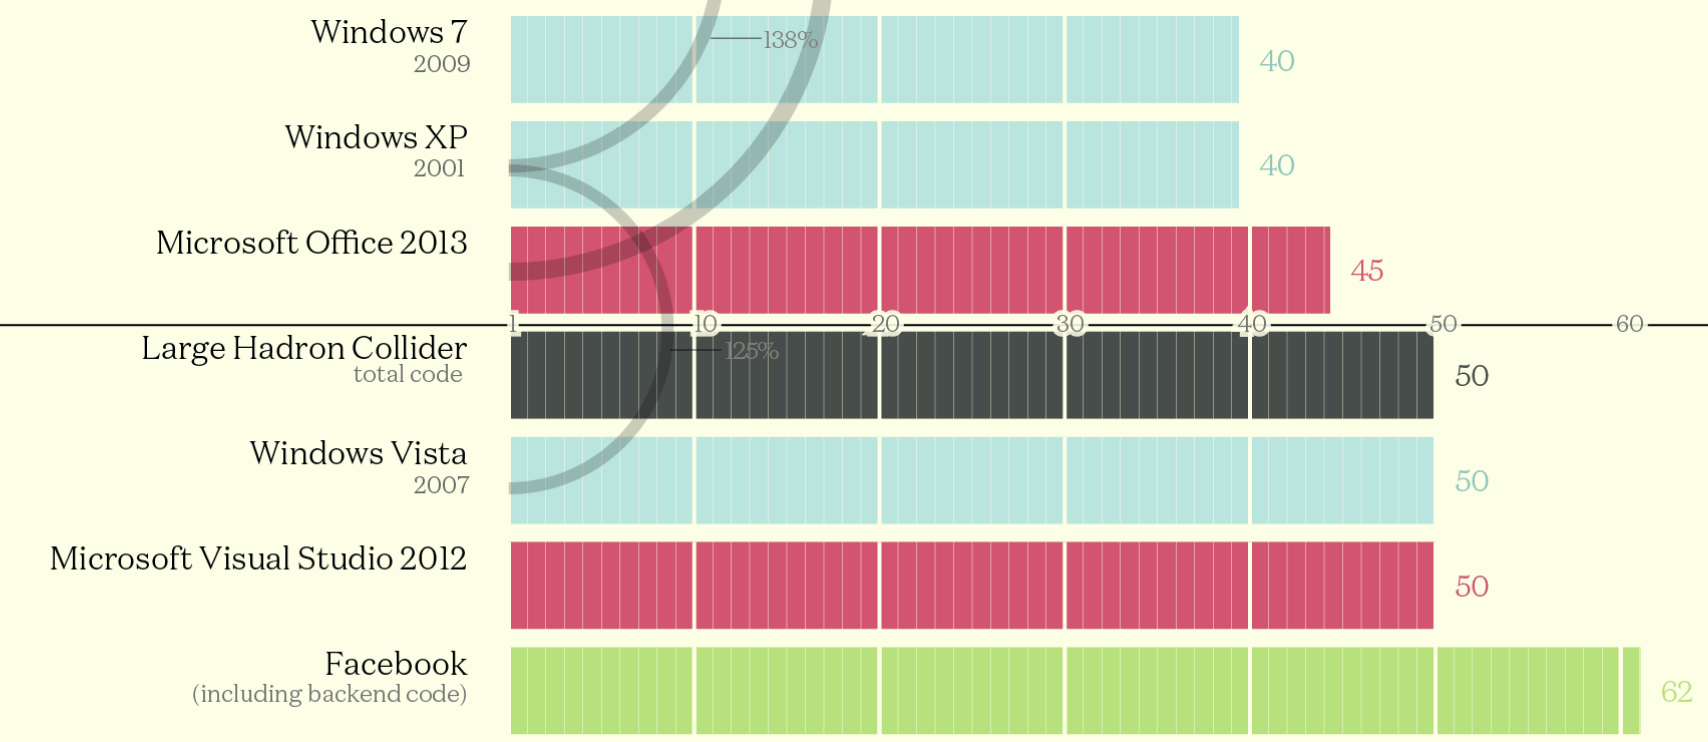
\includegraphics[width=9cm]{ressources/nb-lignes.png}
\captionof{figure}{Infographie complète sur \href{https://www.informationisbeautiful.net/visualizations/million-lines-of-code/}{informationisbeautiful}}
\label{nblignes}
\end{center}
Il est impératif que chaque bloc de code (boucle, fonction...) réalise correctement la tâche qui lui est assignée.
\begin{center}
\shadowbox{\parbox{16cm}{\centering Quels systèmes de contrôle peut-on mettre en place dans un programme informatique?}}
\end{center}
\section{Variant de boucle: terminaison}
\begin{center}
\begin{lstlisting}[language=Python]
i = 10
while i >= 0:
    print(i)
print("Boum")
\end{lstlisting}
\captionof{code}{Boucle infinie}
\label{infinie}
\end{center}
Le code \ref{infinie} ne termine jamais. Nous pouvons supposer que ce n'était pas la volonté initiale du programmeur.
\begin{aretenir}[]
Un \emph{variant de boucle} est une expression dont la valeur varie à chaque itération de la boucle.
\end{aretenir}
Pour chaque boucle construite, il est donc nécessaire de déterminer son \emph{variant} afin de prouver sa \textbf{terminaison}.
\begin{center}
\begin{lstlisting}[language=Python]
i = 10
while i >= 0:
    print(i)
    i = i - 1
print("Boum")
\end{lstlisting}
\captionof{code}{Compte à rebours}
\label{variant}
\end{center}
Dans le code \ref{variant}, \emph{i} est un variant de la boucle: à chaque itération sa valeur décroît de 1, elle deviendra donc négative.
\begin{activite}
L'algorithme \ref{palindrome} permet de déterminer si \emph{mot} est un palindrome.
\begin{center}
\begin{lstlisting}[language=Python]
Fonction: palindrome(mot)
Debut
i = 0
j = longueur(mot) − 1
TantQue i <= j faire
Si mot_i = mot_j alors
	i = i + 1
	j = j − 1
sinon
	Renvoyer Faux
Fin Si
Fin TantQue
Renvoyer Vrai
Fin
\end{lstlisting}
\captionof{code}{Palindrome}
\label{palindrome}
\end{center}
\begin{enumerate}
\item Sur papier, dérouler l'algorithme pour les mots \emph{radar} puis \emph{sauras}.
\item Écrire cet algorithme en Python.
\item Montrer que l'expression $\delta=j-i$ est un variant de la boucle.
\end{enumerate}
\end{activite}
\section{Invariant de boucle: correction}
Une boucle peut terminer mais cependant ne pas réaliser ce à quoi elle est destinée.
\begin{aretenir}[]
Un \emph{invariant de boucle} est une propriété qui si elle est vraie avant l'itération, le reste après son exécution.
\end{aretenir}
\begin{center}
\lstinputlisting[firstline=10,lastline=14]{"scripts/somme-entiers.py"}
\captionof{code}{Somme des premiers entiers}
\label{somme}
\end{center}
Le code \ref{somme} calcule la somme $1+2+...+n$. Nous pouvons montrer par récurrence que l'expression \begin{center}
$s=1+2+...+i-1$
\end{center} est un invariant de la boucle:
\begin{itemize}
\item Avant la première itération, $i=1$ et $s=0$; l'expression est vérifiée.
\item On suppose que la condition est vérifiée au rang \emph{i}.
\item On montre alors qu'elle est vraie au rang $i+1$.
\end{itemize}
\begin{aretenir}[Remarque]
À la dernière itération, $i=n+1$; la boucle n'est alors pas exécutée et l'invariant est bien vérifié:
\begin{center}
$s=1+2+...+(n+1)-1$
\\$s=1+2+...+n$
\end{center}
\end{aretenir}
\begin{activite}
La division de l'entier \emph{a} par l'entier \emph{b} définie par Euclide consiste à trouver deux entiers \emph{q} et \emph{r} tels que 
\begin{center}
$a=q×b+r$
\\avec $0\leq r <b$
\end{center}
Le code \ref{division} détermine ces deux entiers.
\begin{center}
\lstinputlisting[firstline=10,lastline=16]{"scripts/division.py"}
\captionof{code}{Division euclidienne}
\label{division}
\end{center}
\begin{enumerate}
\item Dérouler à la main la fonction pour $a=20$ et $b=6$.
\item Montrer que l'expression $a=q×b+r$ est un invariant de la boucle.
\end{enumerate}
\end{activite}
\section{Préconditions}
Reprenons la fonction \textbf{somme\_des\_entiers} et passons lui le paramètre \emph{-2}.
\begin{center}
\begin{lstlisting}[language=Python]
print(somme_des_entiers(-2))
\end{lstlisting}
\captionof{code}{Somme d'entiers négatifs?}
\label{testneg}
\end{center}
Le résultat est inattendu ou plus exactement il ne correspond pas à ce que nous voudrions obtenir. La fonction telle que nous l'avons écrite n'est adaptée qu'à des valeurs de \emph{n} positives.
\begin{aretenir}[]
Une \textbf{assertion} permet d'effectuer un test et lève une erreur si la condition n'est pas remplie.
\end{aretenir}
\begin{center}
\begin{lstlisting}[language=Python]
def somme_des_entiers(n):
    assert n >= 0, "n doit être positif ou nul"
    s = 0
    for i in range(1, n+1):
        s += i
    return s
\end{lstlisting}
\captionof{code}{Précondition}
\label{assert}
\end{center}
\begin{activite}
Compléter la fonction comme le montre le code \ref{assert} et tester à nouveau le code \ref{testneg}.
\end{activite}
L'erreur levée donne des informations sur le chemin qui a conduit à cette erreur.
\begin{activite}
Une division par zéro est une opération qui n'existe pas. Modifier alors la fonction \textbf{division} pour qu'elle définisse une précondition nécessaire à son exécution.
\end{activite}
\end{Form}
\end{document}